\chapter{Landau-elm\'elet, sk\'al\'az\'as} 
  
 
 \section{Rendparaméter}
   
  A rendparaméter ($\psi$) egy olyan mennyiség, aminek értékével közvetlenül jellemezni tudjuk azt, hogy melyik fázisban vagyunk. $\psi$ egy olyan mennyiség, ami a szimmetrikus fázisban nulla, a szimmetriasértőben pedig véges értéket vesz fel. Legyen $G_{sz}$ a szimmetrikus fázis csoportja, míg $G_{nsz}$ a szimmetriasértőé. Másodrendű az átalakulás, ha $G_{nsz}\subset G_{sz}$, ugyanis ekkor egy paraméter folytonos változtatásával elérhető, hogy a szimmetrikus fázis szimmetriacsoportja $G_{nsz}$-ra szűküljön. Ha $G_{nsz}\nsubseteq G_{sz}$, akkor az átalakulás biztos, hogy elsőrendű.
  
  A rendparaméterhez tartozik egy konjugált tér, mellyel el lehet érni, hogy a szimmetrikus fázisban is véges értéket vegyen fel. Ilyen pl.\ $H$ az FM--PM átalakulásnál, de nincs ilyen valós tér pl.\ az AFM--FM átalakulásnál. 
 
 \section{Landau-elmélet}
 
  A Landau-elmélet alapvető célja, hogy a szabadenergia(-sűrűség)-et felírja mint egy kis paraméter Taylor-soraként a kritikus pont közelében. Ez a kis paraméter a rendparaméter lesz. A ferromágneses--paramágneses átalakulás nyelvezetét használva ($\psi=m$) írjuk fel az elméletet. Az alapfeltevések a következőek:
  \begin{itemize}
   \item $\TC$ környékén a a mágnesezettségi sűrűsége nagyon pici: $m\xrightarrow{T\to\TC}0$,
   \item az állapotok eloszlása nagyon éles $m$ szerint, így az $m$ várható értéke és legvalószínűbb értéke megegyezik,
   \item illetve az eloszlások közelíthetőek Gauss-görbével. (Ez a fluktuációk meghatározásánál lesz hasznos.)
  \end{itemize}
  
  A (mágneses) szabadenergia-sűrűség sorfejtése negyedrendig:
  \al{
   f(T,H,m)=w(T)+\frac{a(T)}{2}m^2+\frac{u(T)}{4}m^4-Hm.
  }
  Mágneses tér nélkül az energia invariáns $m$ előjelétől, így $m$-nek csak páros hatványai szerepelhetnek. Minden hatvány együtthatója függhet $T$-től. Elvárjuk, hogy $u(T)$ pozitív legyen minden $T$-re, hogy létezzen globális minimum. 
  
  Egyensúly ott van, ahol $m$ minimalizálja $f$ értékét:
  \al{
   &0=\pder{f}{m}=a(T)m+u(T)m^3-H
   &0<\pder{^2 f}{m^2}=a(T)+3 u(T)m^2
  }
  
  $H=0$ esetben az $m=0$ jó megoldás. Az egyensúlyi feltétel akkor teljesül, ha $a(T)>0$.
  
  $m\ne 0$ megoldás esetében $m=\sqrt{-\frac{a(T)}{u(T)}}$. Az egyensúlyi feltétel: $0<a(T)+3 u(T)m^2=a(T)-3u(T)\frac{a(T)}{u(T)}=-2a(T)$, tehát itt $a(T)$ negatív. 
  
  Legyen $\TC$ az a hőmérséklet, ahol $a(T)$ előjelet vált. Legegyszerűbb közelítésben $a(T)=a_0(T-\TC)$ és $u(T)=u_0$. Az állapotegyenlet megoldását \aref{fig:B10-landau}. ábra mutatja.
  
  \begin{figure}[ht!]
   \centering
   \subfloat[Az állapotegyenlet megoldása $m(T,H)$-ra.\label{fig:B09-l1}]{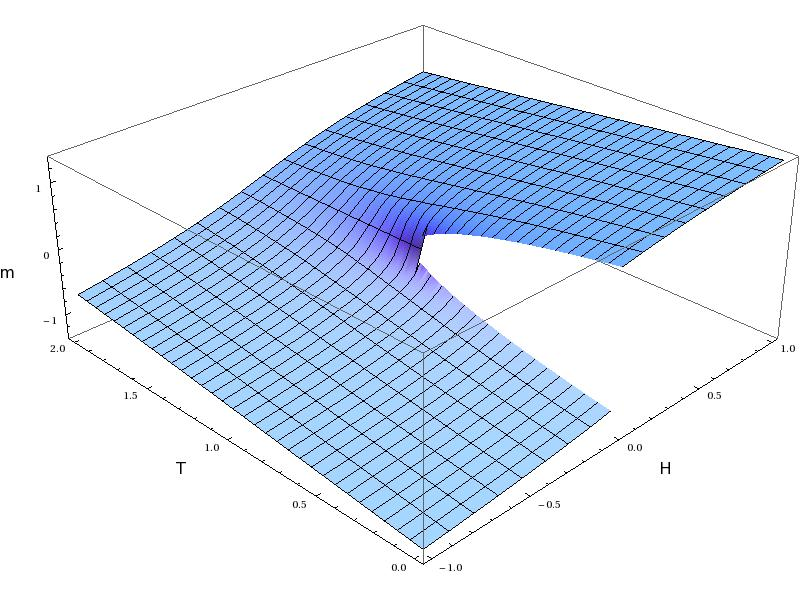
\includegraphics[width= 0.5\textwidth]{./B09tetel/thm}} \\
   \subfloat[Fix mágneses tér mellet az $m(T)$ függvény.\label{fig:B09-l2}]{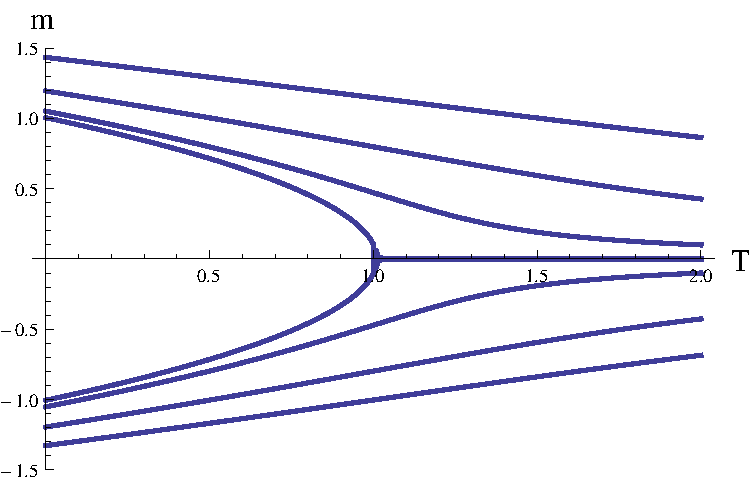
\includegraphics[width= 0.3\textwidth]{./B09tetel/TM}} \hspace{6pt}
   \subfloat[Fix hőmérséklet mellet az $m(H)$ függvény.\label{fig:B09-l3}]{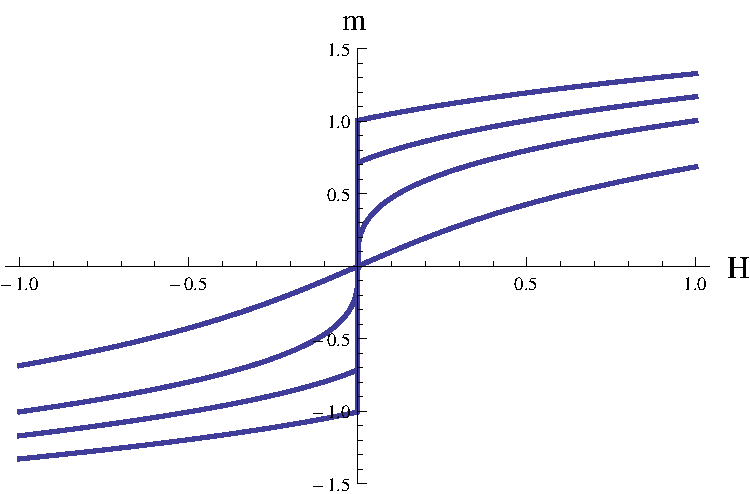
\includegraphics[width= 0.3\textwidth]{./B09tetel/HM}} \hspace{6pt}
   \subfloat[Fix mágnesezettség mellet az $H(T)$ függvény.\label{fig:B09-l4}]{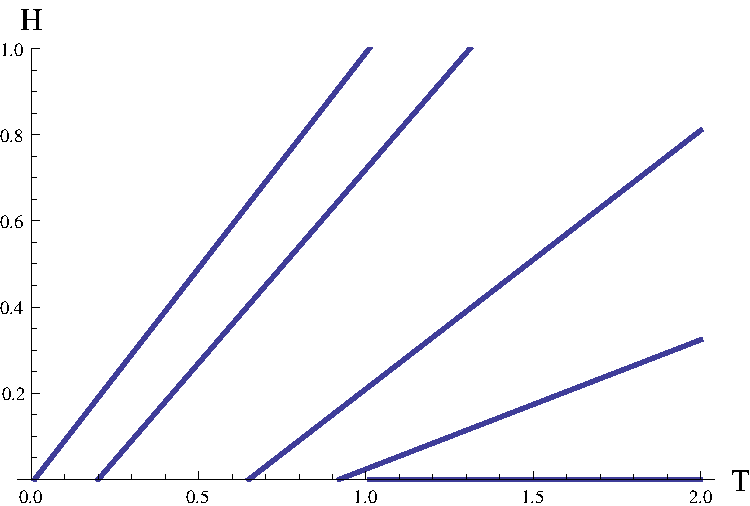
\includegraphics[width= 0.3\textwidth]{./B09tetel/HT}} 
   \caption{A negyedrendű szabadenergia sorfejtéssel felírt Landau-elmélet  állapotegyenlete és annak szintvonalai mindhárom síkra vetítve. Az (a) ábrán látszik, hogy hol hányadrendű az átalakulás: a $H=0$, $T<T_\text{C}$ vonalon $m=\pder{f}{H}$ ugrik, vagyis is elsőrendű az átalakulás, míg $H=0$, $T=T_\text{C}$-ben $m$ érintője, vagyis $\pder{^2 f}{H^2}$ vagy $\pder{^2 f}{H\partial T}$ vagy $\pder{^2 f}{T^2}$ divergál, vagyis az átalakulás abban a pontban másodrendű.}\label{fig:B10-landau}
  \end{figure}
  
  Vezessük be $\tau=T-\TC$-t, a relatív hőmérsékletet.
  Eddig tehát tudjuk, hogy
  \al{
   m=\begin{cases}
      0 & T<\TC\\
      \sqrt{\frac{a_0}{u_0}}\abs{\tau}^{\frac{1}{2}} & T>\TC,
     \end{cases}
  } 
  vagyis $\beta=\frac{1}{2}$.
  
  $T=\TC$-n a mágnesezettség tértől való függését is fel tudjuk írni. Az egyensúlyra vonatkozó egyenletek alapján:
  \al{
   &H=u_0m^3
   &m=\abs{\frac{H}{u}}^{\frac{1}{3}}\sim \abs{H}^\frac{1}{3},
  }
  ahonnan $\delta=\frac{1}{3}$.
  
  Az $m(T)$-ből a szuszceptibilitás, felhasználva az egyensúlyra vonatkozó egyenleteket:
  \al{
   \chi^{-1}=\pder{H}{m}=\pder{^2 f}{m^2}=a(T)+3 u(T)m^2
    =\begin{cases}
      T<\TC: &-2a(T)=2a_0\abs{\tau}\\
      T>\TC: &\phantom{-2}a(T)=a_0\abs{\tau}
     \end{cases}
  }
  vagyis s szuszceptibilitás divergál $T=\TC$-n, csak két oldalról kicsit más együtthatóval. Az exponens $\gamma=1$. 
  
  A szabadenergia az egyensúlyban és $H=0$ esetben:
  \al{
   F(T,H=0)
    &=\min_{M}F(T,H,M)
     =V\min_{m}\left(w(T)+\frac{a(T)}{2}m^2+\frac{u(T)}{4}m^4\right)\\
    &=\begin{cases}
       T<\TC:& V\left(w(T)-\frac{a_0^2\tau^2}{4u_0}\right) \\
       T>\TC:& Vw(T)
      \end{cases}
  }
  A hőkapacitás:
  \al{
   C_V=-T\pder{^2F }{T^2}
    =\begin{cases}
      T<\TC:& -TV\pder{^2 w(T)}{T^2}+TV\frac{a_0^2}{2u_0} \\
      T>\TC:& -TV\pder{^2 w(T)}{T^2}
     \end{cases}
  }
  vagyis $T=\TC$-n a fajhőnek ugrása van: $C(\TC-0)-C(\TC+0)=TV\frac{a_0^2}{2u_0}$, így a fajhő kritikus exponens $\alpha=0$.
  
  A fluktuációk számításához a paramágneses fázisban felhasználjuk, hogy $P(M)\sim e^{-\beta F(T,H,M)}$. $H=0$ esetben, csak a másodrendű tagot megtartva:
  \al{
   &P(M)\sim e^{-\beta V\frac{a(t)}{2}m^2}
   &\Rightarrow
   &&\mv{(\Delta m)^2}&=\frac{1}{\beta V a(T)}=\frac{\kB T}{V a(T)}=\frac{\kB T}{V}\chi\\
   &&&&\mv{(\Delta M)^2}&=\kB T V\chi.
  }
  
  A korrelációs függvény kiszámításához inhomogén mágneses teret és inhomogén mágnesezettséget kell bevezetni. Az $f$-ben $m=m_\text{eq}+\delta m(\rv)$, ahol $\delta m(\rv)$ a helyfüggő kis moduláció a mágnesezettségben. Ekkor a szabadenergia sorfejtésébe bele kell venni az $m(\rv)$ gradiensét is egy $\frac{c}{2}\abs{\grad{m(\rv)}}^2$ taggal. $f$ kifejtve, majd Fourier-transzformálva Gauss-alakú lesz, ahonnan a fluktuáció nagysága leolvasható. Innen a szuszceptibilitás kifejezhető:
  \al{
   &\chi(q)=\frac{1}{c}\frac{1}{q^2+\xi^{-2}}
   &\xi=\sqrt{\frac{c}{a(T)+3u_0m^2}}.
  }
  A korrelációs függvény:
  \al{
   &C(q)=\beta^{-1}\chi(q)
    =\frac{\kB T}{c}\frac{1}{q^2+\xi^{-2}}
   &C(r)=\frac{\kB T}{c}\frac{1}{4\pi}\frac{e^{-r/\xi}}{r},
  }
  így tehát $\xi$ a korrelációs hossz, mely
  \al{
   \xi^{-2}=\frac{1}{c}\big(a(T)+3u_0m^2\big)
    =\begin{cases}
      H=0, T<\TC, \left(m^2=-\frac{a(T)}{u_0}\right): & 2\frac{a_0\abs{\tau}}{c}\\
      H=0, T>\TC, \left(m=0\right): & \frac{a_0\abs{\tau}}{c}\\
      H\ne 0, T=\TC, \left(a=0,H=u_0m^3\right): & \frac{3u_0}{c}\left(\frac{H}{u_0}\right)^{\frac{3}{2}}
     \end{cases}
  }
  Inenn mindjárt látszik, hogy $H=0$-ra $\xi\sim \abs{\tau}^{-\nu}$, $\nu=\frac{1}{2}$. és $T=\TC$-re $\xi\sim \abs{H}^{-\mu}$, $\mu=\frac{1}{3}$. $C(q)$ $\tau=0$ és $H=0$-ra $C(r)\sim r^{-d+2-\eta}$, ahol $d=3$ a dimenziószám, így $\eta=0$.
  
 \section{Ginzburg-kritérium}
  
  A Landau-elmélet dimenziófüggetlen, de a fázisátalakulások nem azok. Nézzük meg, hogy a Landau-elmélet konzisztens-e. 
  
  Számoljuk ki a mágnesezettség fluktuációit:
  \al{
   \mv{\Delta M^2}
   &=\intl{V}{}\drh\intl{V}{}\drkh\mv{m(\rv)-m_\text{eq}}\mv{m(\rv')-m_\text{eq}}
    =\intl{V}{}\drh\intl{V}{}\drkh C(\rv-\rv')\\
   &=V\intl{V}{}\drh C(\rv)
    =VC(q=0)
    =V\kB T \chi(q=0)
    =V\kB T \chi
  }
  A relatív fluktuáció:
  \al{
   \frac{\mv{\Delta M^2}}{M^2}
    =\frac{V\kB T \chi}{M^2}
    =\frac{\kB T \chi}{V m^2}.
  }
  A korrelációk csak $\xi^d$ tartományban vannak, így a minta térfogata helyett ebben a térfogatban tekintsük a relatív fluktuációkat. Ekkor a hőmérséklettől való függés:
  \al{
   \frac{\mv{\Delta M^2}}{M^2}
    =\frac{\kB T \chi}{\xi^d m^2}
    \sim\frac{\abs{\tau}^{-1}}{\abs{\tau}^{-d/2}\cdot\abs{\tau}^{2\cdot 1/2}}
    \sim \abs{\tau}^{d/2-2}.
  }
  Az elmélet akkor használható, ha $\tau\to 0$-re a szabadenergia-sűrűség sorfejtése értelmes, azaz, ha a fluktuációk nem robbannak fel. Ehhez szükséges, hogy $d/2-2\ge 0$, vagyis $d\ge 4$. Tehát a Landau-elmélet szigorúan véve csak négy, vagy annál nagyobb dimenzióban értelmes.
  
  Praktikusan ez alacsony dimenzióban a Landau-elméletnek egy korlátot ad, hogy meddig érvényes. Annyira közelíthetjük meg $\TC$-t, hogy ez a fluktuációs tag még $\sim\mathcal{O}(1)$ legyen.
  
 \section{Skálahipotézis, skálázás}
  
  A sálahipotézis abból, áll, hogy feltesszük, hogy a rendszerben egyetlen karakterisztikus hosszúság van, a korrelációs hossz. 
  
  A korrelációs függvény ekkor: $C(q,\xi)=C(q=0,\xi)\cdot\phi(q\xi)$, ugyanis másképp nem függhet $q$-tól. Tudjuk, hogy $C(q=0)\sim\chi\sim\abs{\tau}^{-\gamma}$, illetve $\xi\sim\abs{\tau}^{-{\nu}}$, így $C(q=0)\sim\xi^{\frac{\gamma}{\nu}}$, vagyis
  \al{
   C(q,\xi)=\xi^{\frac{\gamma}{\nu}}\cdot\phi'(q\xi).
  }
  Ez egy általánosított homogén függvény, hiszen
  \al{
   &C\left(\lambda q,\frac{\xi}{\lambda}\right)
    &=\left(\frac{\xi}{\lambda}\right)^{\frac{\gamma}{\nu}}\phi'\left(\lambda q\frac{\xi}{\lambda}\right)
     =\lambda^{-\frac{\gamma}{\nu}}C\left(q,\xi\right)
   &\Rightarrow
   &&C\left(q,\xi\right)=\lambda^{\frac{\gamma}{\nu}}C\big(\lambda q,\lambda^{-1}\xi\big).
  }
  Visszaírva a $\tau$ függést: $\xi=\xi_0\abs{\tau}^{-\nu}$ $\rightarrow$ $\lambda^{-1}\xi=\xi_0\left(\lambda^{\frac{1}{\nu}}\abs{\tau}\right)^{-\nu}$, vagyis $C(q,\tau)=\lambda^{\frac{\gamma}{\nu}}C\big(\lambda q,\lambda^{\frac{1}{\nu}}\tau\big)$. 
  
  Teljesen hasonlóan le lehet vezetni a $H$-tól való függést $\xi$-n keresztül. Összegezve:
  \al{
   C\left(q,\tau,H\right)=\lambda^{\frac{\gamma}{\nu}}C\Big(\lambda q,\lambda^{\frac{1}{\nu}}\tau,\lambda^{\frac{1}{\mu}}H\Big),
  }
  ami még mindig egy hipotézis, csak jól argumentált. 
  A korrelációs függvényre hasonló skálahipotézis adható. Ez úgy adható meg, hogy $\xi$ az a távolság ami alatt a korrelációs függvény a felére csökken: $C(q=\frac{1}{\xi})=\frac{1}{2}C(q=0)$, ennek kifejtéséből:
  \al{
   \xi(\tau,H)=\lambda \xi\Big(\lambda^{\frac{1}{\nu}}\tau,\lambda^{\frac{1}{\mu}}H\Big).
  }
  A korrelációs függvényre vonatkozó skálahipotézisből a szuszceptibilitás ($\chi=\beta C(q=0)$): $\chi(\tau,H)=\lambda^{\frac{\gamma}{\nu}}C\big(\lambda^{\frac{1}{\nu}}\tau,\lambda^{\frac{1}{\mu}}H\big)$, ahol $\lambda'=\lambda^{\frac{1}{\nu}}$-t bevezetve
  \al{
   \chi(\tau,H)=\lambda^{\gamma}\chi\Big(\lambda\tau,\lambda^{\frac{\nu}{\mu}}H\Big). 
  }
  A mágnesezettség: $\chi=\pder{m}{H}$, vagyis akkor 
  \al{
   m(\tau,H)=\lambda^{\gamma-\frac{\nu}{\mu}}m\Big(\lambda\tau,\lambda^{\frac{\nu}{\mu}}H\Big)
  }
  kell, hogy legyen. Hasonlóan a szabadenergia-sűrűség:
  \al{
   f(\tau,H)=\lambda^{\gamma-2\frac{\nu}{\mu}}f\Big(\lambda\tau,\lambda^{\frac{\nu}{\mu}}H\Big).
  }
  
  \subsection{Összefüggések a kritikus exponensek között}
   \begin{itemize}
    \item A korrelációs hossz, ha $H=0$, és $\lambda=\abs{\frac{\tau}{\tau_0}}^{-\nu}$:
    \al{
     \xi(\tau,0)
      =\lambda \xi\Big(\lambda^{\frac{1}{\nu}}\tau,0\Big)
      =\abs{\frac{\tau}{\tau_0}}^{-\nu} \xi\left(\abs{\frac{\tau}{\tau_0}}^{\frac{-\nu}{\nu}}\tau,0\right)
      =\abs{\frac{\tau}{\tau_0}}^{-\nu} \underbrace{\xi\Big(\pm\tau_0,0\Big)}_{=\text{konst}}
      \sim \abs{\tau}^{-\nu},
    }
    illetve ha $\tau=0$ és $\lambda=\abs{\frac{H}{H_0}}^{-\mu}$:
    \al{
    \xi(0,H)
     =\lambda \xi\Big(0,\lambda^{\frac{1}{\mu}}H\Big)
     =\abs{\frac{H}{H_0}}^{-\mu} \xi\left(0,\abs{\frac{H}{H_0}}^{\frac{-\mu}{\mu}}H\right)
     =\abs{\frac{H}{H_0}}^{-\mu} \underbrace{\xi\left(0,\pm H_0\right)}_{=\text{konst}}
     \sim \abs{H}^{-\mu}.
    }
    
    \item A szuszceptibilitás $H=0$-ra és $\lambda=\abs{\frac{\tau_0}{\tau}}$-t választva:
    \al{
     \chi(\tau,0)
      =\lambda^{\gamma}\chi\Big(\lambda\tau,0\Big)
      =\abs{\frac{\tau_0}{\tau}}^{\gamma}\chi\Big(\abs{\frac{\tau_0}{\tau}}\tau,\lambda^{\frac{\nu}{\mu}}H\Big)
      =\abs{\frac{\tau_0}{\tau}}^{\gamma}\underbrace{\chi\Big(\pm\tau_0,0\Big)}_{=\text{konst}}
      \sim\abs{\tau}^{-\gamma}
    }
    
    \item A korrelációs függvény $\tau=0$ és $H=0$-ra, $\lambda=\frac{q_0}{q}$ választással
    \al{
     C\left(q,0,0\right)
      =\lambda^{\frac{\gamma}{\nu}}C\Big(\lambda q,0,0\Big)
      =\left(\frac{q_0}{q}\right)^{\frac{\gamma}{\nu}}C\left(\frac{q_0}{q} q,0,0\right)
      =\left(\frac{q_0}{q}\right)^{\frac{\gamma}{\nu}}\underbrace{C\left(q_0,0,0\right)}_{=\text{konst}}
      \sim q^{-\frac{\gamma}{\nu}}.
    }
    Az $\eta$ kritikus exponenst úgy definiáltuk, hogy $C(q)\sim q^{-2+\eta}$, így $-2+\eta=-\frac{\gamma}{\nu}$ azonnal adódik.
    
    \item A mágnesezettségi sűrűségből $H=0$ esetben $\lambda=\abs{\frac{\tau_0}{\tau}}$-t választva:
    \al{
     m(\tau,0)
      =\lambda^{\gamma-\frac{\nu}{\mu}}m\Big(\lambda\tau,0\Big)
      =\abs{\frac{\tau_0}{\tau}}^{\gamma-\frac{\nu}{\mu}}m\Big(\abs{\frac{\tau_0}{\tau}}\tau,0\Big)
      =\abs{\frac{\tau_0}{\tau}}^{\gamma-\frac{\nu}{\mu}}\underbrace{m\Big(\pm\tau_0,0\Big)}_{=\text{konst}}
      \sim \abs{\tau}^{-\gamma+\frac{\nu}{\mu}}.
    }
    Szintén a korábbi $\beta$ exponens definíciójából $\beta=-\gamma+\frac{\nu}{\mu}$. Hasonlóan $\tau=0$, $
    \lambda=\abs{\frac{H_0}{H}}^{-\frac{\mu}{\nu}}$.
    \al{
     m(0,H)
      &=\lambda^{\gamma-\frac{\nu}{\mu}}m\Big(0,\lambda^{\frac{\nu}{\mu}}H\Big)
      =\abs{\frac{H_0}{H}}^{-\frac{\mu}{\nu}\gamma+1}m\Big(0,\abs{\frac{H_0}{H}}H\Big)
      =\abs{\frac{H_0}{H}}^{-\frac{\mu}{\nu}\gamma+1}\underbrace{m\Big(0,\pm H_0\Big)}_{=\text{konst}}\\
      &\sim\abs{H}^{\frac{\mu}{\nu}\gamma-1}.
    }
    Szintén a korábbi definícióval való összevetésből: $\frac{1}{\delta}=-\frac{\mu}{\nu}\gamma+1$.
    
    \item Végül a fajhőhöz $f$, ha $H=0$: válasszuk $\lambda=\abs{\frac{\tau_0}{\tau}}$,
    \al{
     f(\tau,0)
     &=\lambda^{\gamma-2\frac{\nu}{\mu}}f\Big(\lambda\tau,0\Big)
      =\abs{\frac{\tau_0}{\tau}}^{\gamma-2\frac{\nu}{\mu}}f\Big(\abs{\frac{\tau_0}{\tau}}\tau,0\Big)
      =\abs{\frac{\tau_0}{\tau}}^{\gamma-2\frac{\nu}{\mu}}\underbrace{f\Big(\pm\tau_0,0\Big)}_{=\text{konst}}
      \sim \abs{\tau}^{-\gamma+2\frac{\nu}{\mu}}.
    }
    Innen a fajhő $\tau$ függése megadható, hiszen az a szabadenergia-sűrűség második deriváltjával arányos. A két deriválás a kitevőben $-2$-t hoz be, így $C\sim\pder{^2 f}{T^2}\sim \abs{\tau}^{-\gamma+2\frac{\nu}{\mu}-2}$. A korábbi definíció alapján így: $\alpha=\gamma-2\frac{\nu}{\mu}+2$. Ennek az egyenlőségnek az átírásához felhasználjuk a $\beta$-ra vonatkozó egyenletet: $\alpha=-2\beta-\gamma+2$.
   \end{itemize}
   
   Összefoglalva:
   \al{
     C&\sim\abs{\tau}^{-\alpha} && H=0\\
     m&\sim\abs{\tau}^{\beta} && H=0\\
     \chi&\sim\abs{\tau}^{-\gamma} && H=0\\
     m&\sim\abs{H}^{\frac{1}{\delta}} && \tau=0\\
     \xi&\sim\abs{\tau}^{-\nu} && H=0\\
     \xi&\sim\abs{H}^{-\mu} && \tau=0\\
     C(q)&\sim \frac{1}{q^{2-\eta}} \;\Leftrightarrow \; C(r)\sim \frac{1}{r^{d-2+\eta}}&& \tau=0,H=0,
   }
   illetve a skálatörvények:
   \al{
    &\gamma=\nu(2-\eta)
    &\beta=-\gamma+\frac{\nu}{\mu}
    &&\frac{1}{\delta}=\frac{\nu-\mu\gamma}{\nu}
    &&2-\alpha=2\beta+\gamma.
   }
   Tehát $\gamma,\mu,\nu$-vel ki lehet fejezni az összes exponenst. Ez a három exponens határozza meg az univerzalitási osztályokat. 
   \paragraph{Hiperskálatörvény}
    
    Ezeken felül még egy skálatörvény belátható, ami a dimenziószámot is figyelembe veszi. A Ginzburg-kritériumnál láttuk, hogy 
    \al{
     \frac{\mv{\Delta M^2}}{M^2}
    =\frac{\kB T \chi}{V m^2}.
    }
    
    Azt láttuk, hogy egy korrelációs hossznyi tartományban ez csak akkor nem divergál $T\to\TC$-re, ha $d\ge 4$. Ha ez mégis divergálna, akkor létezne egy nagyobb térfogat, $R^d$, ahol a relatív fluktuáció $\sim\mathcal{O}(1)$. De ez ellentmondás, mert a skálahipotézis kimondja, hogy nem létezik más karakterisztikus távolság, csak $\xi$, úgyhogy annak kell igaznak lennie, hogy 
    \al{
    \mathcal{O}(1)\sim
     \frac{\kB T \chi}{\xi^d m^2}
     \sim\frac{\abs{\tau}^{-\gamma}}{\abs{\tau}^{-d\nu}\cdot\abs{\tau}^{2\cdot \beta}}
    \sim \abs{\tau}^{d/\nu-2\beta-\gamma},
    }
    vagyis $d/\nu-2\beta-\gamma=0$, ahonnan a hiperskálatörvény:
    \al{
     d\nu=2\beta+\gamma.
    }
    Az Ising-exponensekkel így az jön ki, hogy a Landau-elmélet csak $d=4$ dimenzióban korrekt.
    
 
 \section{Univerzalitás}\label{ss:B10-univerzalitas}
  
  A másodrendű fázisátalakulások rengeteg rendszerben jelen vannak. A megfigyelés az, hogy látszólag teljesen különböző rendszerek is ugyanazt a viselkedést mutatják a kritikus pont közelében. 
  
  Ennek magyarázata az, hogy ahogy a rendszer egyre közelebb kerül a kritikus ponthoz, úgy az egyre inkább skálafüggetlenné válik. Emiatt a rendszernek minden skáláfüggő tulajdonsága elvész, és csak a néhány releváns, skálafüggetlen tulajdonság marad. 
  
  A kritikus pont közelében a rendszerek hasonlósága abban nyilvánul meg, hogy a kritikus exponensek megegyeznek. Ez alapján a hasonló rendszereket univerzalitási osztályokba lehet sorolni. Az XY-osztályba tartozik például az az XY-Heisenbeg-model, a szupravezetés és a szuperfolyékonyság; az Ising-osztályba tartozik az Ising-modell, a folyadék--gáz fázisátalakulások és az uniaxiális mágnesek. A Heisenberg-osztályba az izotrop mágnesek és a Heisenberg-modell. 
  
  
  